\begin{comment}
\section{Osservabili stellari/demo beamer}

\begin{frame}<1>[label=noinside]{Modello stellare}{Come indagare la fisica interna a una stella?}

\onslide<1->\begin{block}{Osservabili stellari:}
$L$, $M$, $R$, $T_e$, $(\frac{Z}{X})_{ph}$, $g_{ph}$.
\end{block}

\onslide<1->\begin{block}{Informazioni sulla struttura interna?} Condizione di equilibrio idrostatico
\end{block}

%Teorema Vogt-Russel: $X_i(r)$, $M$ \pause equilibrio (idrostatico/termico) determinano struttura stellare .
%\pause

\onslide<1->\begin{block}{Modello stellare: diagramma di \hr{}.}
\end{block}

\onslide<2->\begin{block}{Descrizione fisica interno stellare: parametri aggiuntivi}
Convezione, diffusione e sedimentazione elementi pesanti, equazione di stato, opacit\'a
\end{block}

\onslide<2->\begin{block}{Astrosismologia}
Restringo spazio parametri sistemi stellari lontani
\end{block}

\end{frame}

{ % all template changes are local to this group.
    \set
\section{beamer}
template{navigation symbols}{}
    \begin{frame}[plain]{Diagramma di \hr{}}
        \begin{tikzpicture}[remember picture,overlay]
            \node[at=(current page.center)] {
                %\includegraphics[width=\paperwidth]{yourimage}
            };
        \end{tikzpicture}
     \end{frame}
}
\againframe<2>{noinside}

\section{Inversione della legge di Duvall}

\section{Inversione non asintotica}

\section{Vincoli al modello solare dalle osservazioni sismologiche}

\end{comment}

\begin{frame}<presentation:0>[noframenumbering]{Problema inverso}

\begin{itemize}

\item diverso comportamento delle autofunzioni

\item Inversione legge di Duvall. valida nelle regioni in cui le autofunzioni variano molto pi\'u rapidamente delle grandezze di equilibrio

per i modi pi\'u penetranti nell'interno solare la perturbazione del potenziale gravitazionale influenza sensibilmente $F(\frac{\omega}{L})$ mentre per modi confinati vicino alla superficie $\alpha$ dipende da l.

%L'inversione del sistema completo di equazioni dei modi si effettua considerando le perturbazioni al MSS che danno un miglior accordo tra frequenze osservate e misurate: considero solo i termini lineari nelle perturbazioni e quindi le correzioni agli autovettori sono trascurate.

\item l'accuratezza della struttura del \mss{} , in particolare del profilo radiale della velocit\'a del suono, della densit\'a e di $\Gamma_1$.
  
\end{itemize}

\end{frame}

\section{Inversione della legge di Duvall.} % 


\subsection{Inversione analitica della velocit\'a del suono}

\begin{frame}{Inversione analitica velocit\'a del suono}
\begin{minipage}{0.65\textwidth}
\begin{figure}[!ht]
        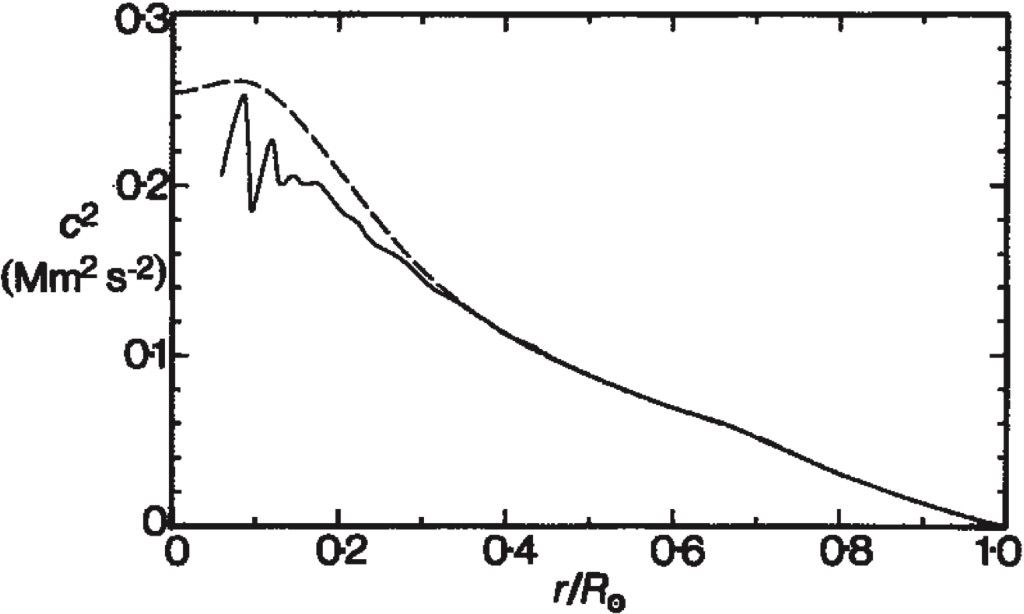
\includegraphics[width=0.54\textwidth,keepaspectratio]{soundspeed}
\end{figure}
\end{minipage}
~
\begin{minipage}{0.3\textwidth}
\captionof{figure}{Profilo radiale di $c_s^2$ determinato invertendo la legge di Duvall dalle frequenze osservate. Da \cite{christensen1985speed}.}\label{fig:soundspeedccm}
\end{minipage}


%\begin{align}
%&F(w)=\int_{r_t}^R\sqrt{1-\frac{c_s^2}{r^2w^2}}\,\frac{dr}{c_s}\label{eq:duvallf}\\
%&(n+\alpha)\pi\approx\int_{r_t}^Rk_r\,dr\approx\int_{r_t}^R\frac{\omega}{c_s}\sqrt{1-\frac{S_l^2}{\omega^2}}\,dr%\label{eq:duvallexpli}
%\end{align}

\begin{equation}
r=R\Exp{-\frac{2}{\pi}\int_{a_s}^a(w\expy{-2}-a\expy{-2})\expy{-\frac{1}{2}}\TDy{w}{F}\,dw}\label{eq:analinversionc}
\end{equation}
dove $a=\frac{c_s}{r}$.

errore sistematico dovuto alla tecnica di inversione nel range $0.4\leq x \leq 0.9$ \'e minore del $2.5\%$.

\end{frame}


\subsection{Struttura dei modi penetranti nel core stellare}

\begin{frame}{Effetti evoluzione sulla separazione dei modi}


%La deviazione dalla \eqref{eq:freqequi} fornisce informazioni sull'evoluzione chimica del core di fusione: infatti estendendo ancora l'espansione di \eqref{eq:duvallf} si ha una misura della variazione di $c_s$ nel core della stella
\begin{equation}\label{eq:tassoul}
    d_{nl}=\nu_{nl}-\nu_{n-1,l+2}\approx-(4l+6)\frac{\Delta\nu}{4\pi^2\nu_{nl}}\int_0^R\frac{dc_s}{dr}\frac{dr}{r}
\end{equation}
%La velocit\'a del suono \'e ridotta a causa dell'aumentare di $\mu$ durante la fusione di H in He durante l'evoluzione stellare: il centro solare \'e un minimo locale per la velocit\'a del suono e quindi, essendo il gradiente della velocit\'a del suono positivo, la parte centrale da un contributo sempre pi\'u negativo in \eqref{eq:tassoul} con l'evolversi della stella.

\end{frame}


%\subsection{Forma differenziale della legge di Duvall}

\begin{frame}<handout:0 beamer:0>{Legge Duvall diferenziale}

Considero l'effetto di perturbazioni del modello sulle frequenze dei modi:
\begin{equation}
S_{nl}\frac{\delta\omega_{nl}}{\omega_{nl}}\approx H_1(\frac{\omega_{nl}}{L})+H_2(\omega_{nl})\label{eq:Dlinear}
\end{equation}

\begin{align}
&S_{nl}=\int_{r_t}^R(1-\frac{L^2c^2}{r^2\omega_{nl}^2})\expy{-\frac{1}{2}}\frac{dr}{c}-\pi\TDy{\omega}{\alpha}\\
&H_1(w)=\int_{r_t}^R(1-\frac{c^2}{r^2w^2})\expy{-\frac{1}{2}}\frac{\delta_rc}{c}\frac{dr}{c},\ H_2(\omega)=\frac{\pi}{\omega}\delta\alpha(\omega)
\end{align}

La funzione $S_{nl}$ \'e approssimabile con un temine proporzionale a $Q_{nl}$ (\cite{christensen1991solar}):
\begin{align}
&\frac{S_{nl}}{\tau_0}\approx Q_{nl}\\
&\tau_0=\int_{0}^R\frac{dr}{c_s}
\end{align}

%Le differenze nella velocit\'a del suono nelle varie regioni influiscono sulle differenze nelle frequenze con un peso dato dal tempo impiegato da un'onda sonora ad attraversare la regione: le differenze nella regione vicino alla superficie dove $c_s$ \'e minore hanno un effetto relativamente grande sulle differenze di frequenza.
\end{frame}

\begin{frame}<handout:0 beamer:0>{Inversione di $H_1$ e $h_2$}

La relazione \eqref{eq:Dlinear}, considerando che $1-\midfrac{L^2c^2}{r^2\omega^2}\approx1$ ad eccezione delle regioni vicino al punto d'inversione $r_t$, pu\'o essere approssimata da
\begin{equation}
\frac{\delta\omega}{\omega}\approx\frac{\int_{r_t}^{R}\frac{\delta_rc_s}{c_s}\frac{dr}{c_s}}{\int_{r_t}^R\frac{dr}{c_s}}
\end{equation}

Una volta determinato $H_1$ le differenze nel profilo radiale di $c_s$ sono determinate tramite
\begin{equation}
\frac{\delta_rc_s}{c_s}=-\frac{2a}{\pi}\TDof{\ln{r}}\int_{a_s}^a(a^2-w^2)\expy{-\frac{1}{2}}H_1(w)\,dw
\end{equation}

Le funzioni $H_1(\frac{\omega_{nl}}{L})$ e $H_2(\omega_{nl})$ possono essere ottenute separatamente attraverso fitting dei dati sperimentali: la prima caratterizza il contributo alle differenze nelle frequenze dei modi dovuto alle differenze del profilo radiale della velocit\'a del suono, la seconda alle diffenze nella regione vicino alla superficie.

\end{frame}

\begin{frame}<handout:0 beamer:0>{Differenze idrogeno/zona ionizzazione}

\begin{figure}[!ht]
        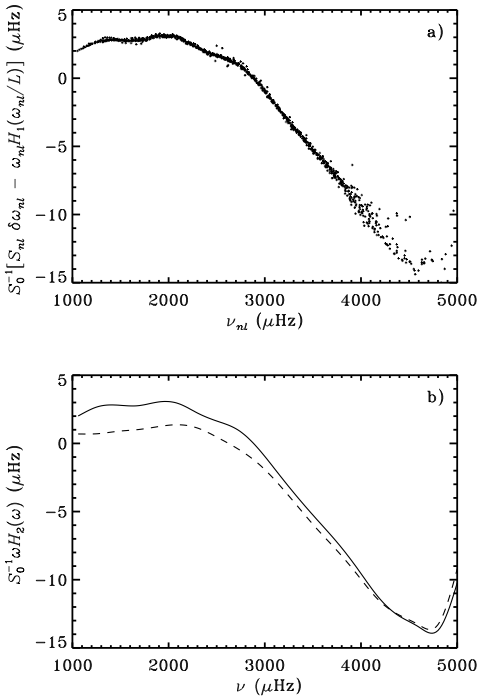
\includegraphics[width=0.34\textwidth,keepaspectratio]{H2dnd}
        \caption{a) Residuo della differenza di frequenze fra il sole e un modello senza diffusione a cui \'e stato sottratto $H_1$. b) Fit di $H_2$ linea continua e per contrasto fit di $H_2$ per differenze di frequenze tra Sole e modello con diffusione. Da \cite{dal03notes}.}\label{fig:H2dnd}
\end{figure}

\end{frame}



\begin{frame}<handout:0 beamer:0>{Regioni superficiali}

La funzione $H_2$ \'e determinata dalla regione sotto la fotosfera. \cite{chr92phase}, analizzando la relazione tra $H_2(\omega)$ e le differenze in $c_s(r)$ e $\Gamma_1$ nelle regioni esterne, hanno visto che discrepanze pi\'u vicino alla superficie generano una componente lentamente oscillante in $H_2(\omega)$ e la ''frequenza'' aumenta con l'aumentare della profondit\'a. \'E inoltre possibile indagare l'andamento di $\Gamma_1$ nella regione di seconda ionizzazione di He e pi\'u in generale il comportamento di $H_2(\omega)$ nelle zone di ionizzazione di H e He consente un'analisi dell'equazione di stato e determinazione dell'abbondanza di elio nella zona convettiva. In figura \ref{fig:H2dnd} si mostra le differenze nelle frequenze tra il Sole ed un modello che non considera la diffusione degli elementi: l'andamento oscillatorio della linea continua nel pannello b \'e dovuto alla differenza nell'abbondanza di idrogeno negli strati superficiali.

\end{frame}


\section{Inversione non asintotica.} % Inizio chapter "Inversione non asintotica." senza nuava pagina

\begin{frame}{Inversione non asintotica}

%La soluzione del problema inverso per il sistema completo di equazioni si basa sulla linearizzazione delle variazioni attorno ad un modello di cui siano calcolabili le autofunzioni dell'operatore $L$ definito in \eqref{eq:variational}.

Utilizzo la formula \eqref{eq:variational} specializzata al problema dell'inversione delle differenze $\delta\omega_{nl}=\omega_{\odot}-\omega_{Mod}$ fra frequenze osservate e predette da un modello. Per l'inversione della struttura idrostatica si ha:
\begin{align}
&\frac{\delta\omega_{nl}}{\omega_{nl}}=\int_0^R[K^{nl}_{c^2,\rho}(r)\frac{\delta_rc^2}{c^2}(r)+K^{nl}_{\rho,c^2}(r)\frac{\delta_r\rho}{\rho}(r)]\,dr+I_{nl}\expy{-1}F_{Surf}(\omega_{nl})+\sigma_i\label{eq:invstructure}\\
&\frac{\delta_rc^2}{c^2}(r)=\frac{[c_{\odot}^2(r)-c_{mod}^2(r)]}{c^2(r)},\ \frac{\delta_r\rho}{\rho}(r)=\frac{[\rho_{\odot}(r)-\rho_{mod}(r)]}{\rho(r)}
\end{align}

\end{frame}

%E quindi si determinano attraverso procedure numeriche le correzioni alla struttura del modello sulla base delle differenze tra frequenze dei modi. Il peso che una perturbazione ha sulla differenze in frequenza \'e determinato dalle autofunzioni dei modi calcolate tramite un modello solare.
%Asymptotic approximation for radial eigenfunction (integral equation connectin sound speed $c(r)$ to $\Omega_{nl}$) is inadequate (especially in deep interior)

\begin{frame}{incertezze inversione non asintotica}

%In \ref{fig:deltacwu} la banda chiara attorno allo zero, che indica il modello solare in perfetto accordo con le osservazioni sismologiche, mostra l'incertezza nell'inversione della velocit\'a del suono; essa \'e dovuta a

\begin{itemize}

\item Incertezze nelle frequenze dei modi osservate.%Oltre all'incertezza statistica propria del determinato strumento \'e possibile valutare gli effette di eventuali
Errori sistematici confrontando i risultati dell'inversione per set di frequenze ottenute con strumenti diversi: la differenza nella velocit\'a del suono \'e minore di $0.02\%$.

\item Incertezze inerenti la tecnica di inversione.

\item Incertezze legate alla dipendenza da un modello solare per il calcolo dei kernel in \eqref{eq:invstructure}.%, \eqref{eq:invdGammadrho}, \eqref{eq:splitfreqrotation}.

\end{itemize}

\end{frame}

\subsection{Tecniche di inversione numeriche.}
%vedi JCD 2002 pg 25-32


\subsubsection{RLS}

\begin{frame}{RLS}

Usando la tecnica del minimo $\chi^2$ regolarizzato si parametrizza la funzione incognita $\frac{\delta f}{f}$ tramite funzioni di base opportune.

La funzione da minimizzare \'e
\begin{equation}
Y=(N-N_p)\chi^2+\alpha N\int_0^1(x\TDof{x}\frac{\Delta f}{f})^2\,dx\label{eq:minimizerls}
\end{equation}
con
\begin{equation}
\chi^2=\frac{1}{N-N_p}\sum_{\alpha=1}^N(\frac{\delta\omega_{obs}-\delta\omega_{fit}}{\sigma})^2_{\alpha}
\end{equation}
%N indica il numero totale di modi $\alpha$, $N_p$ il numero di parametri da determinare, $\Delta\nu_{fit}$, ricavato tramite \eqref{eq:variational}, contiene la funzione incognita opportunamente parametrizzata; il secondo addendo del lato destro di \eqref{eq:minimizerls} \'e introdotto per ridurre oscillazioni indesiderate nel risultato dell'inverisone con $\alpha$, parametro di regolarizzazione, scelto opportunamente.

\end{frame}

\subsubsection{Subtractive Optimally Localized Averaging}

\begin{frame}{SOLA}

Scelgo dei coefficienti $c_i(r_0)$ tali che $\sum c_i(r_0)\frac{\delta\omega_i}{\omega_i}$ fornisca una media del valore di $\frac{\delta f(r)}{f(r)}$ in $r=r_0$:

\begin{equation}\label{eq:SOLAfmean}
\sum_ic_i(r_0)\frac{\delta\omega_i}{\omega_i}=\int_0^R\sum_ic_i(r_0)K^i(r)\frac{\delta f(r)}{f(r)}\,dr=\exv{\frac{\delta f(r_0)}{f(r_0)}}
\end{equation}

e i coefficienti $c_i(r_0)$ sono determina minimizzando la funzione

\begin{equation}\label{eq:SOLAcir0min}
\int_0^R[\mathcal{K}(r_0,r)-\mathcal{T}(r_0,r)]^2\,dr+\mu\sum_i\sigma_ic_i(r_0)c_j(r_0)
\end{equation}
con $\mathcal{K}(r_0,r)=\sum_ic_i(r_0)K^i(r)$ e la funzione target $\mathcal{T}(r_0,r)$, la cui larghezza \'e anch'essa parametro del fit, determina la natura precisa della localizzazione.

\end{frame}


\begin{frame}<presentation:0>[noframenumbering]{Determinazione variazioni velocit\'a del suono}

%Illustro la tecnica SOLA per determinare $\frac{\delta_rc^2}{c^2}$: si formano delle combinazioni lineari di $\frac{\Lvar{\omega_i}}{\omega_i}$ pesate da coefficienti $c_i(r_0)$ tali che $\frac{\Lvar{c^2}}{c^2}$ sia centrato attorno $r_0$ e che gli altri termini in \eqref{eq:invstructure} siano soppressi, queste compongo un averaging kernel $\mathcal{K}_{c^2,\rho}(r_0,r)=\sum_ic_i(r_0)K_{c^2,\rho}^i(r)$, con $\int_0^R\mathcal{K}(r_0,r)\,dr=1$.

%Determino i coefficienti minimizzando l'espressione
\begin{align*}
&\int_0^R[\mathcal{K}_{c^2,\rho}(r_0,r)-\mathcal{T}(r_0,r)]^2\,dr+\beta\int_0^R\mathcal{L}_{\rho,c^2}(r_0,r)\,dr\\
&+\mu\sum_i\sigma_ic_i(r_0)c_j(r_0)
\end{align*}
I contributi indesiderati di $\frac{\delta_r\rho}{\rho}$ sono controllati da:
\begin{equation}
\mathcal{L}_{\rho,c^2}(r_0,r)=\sum_ic_i(r_0)K_{\rho,c^2}^i(r)
\end{equation}

%Il primo termine approssima il valore di $\frac{\delta c^2}{c^2}$ pesato dal kernel $\mathcal{K}(r,r_0)=\sum_ic_i(r_0)K_{c^2,\rho}^i(r)$
%,l secondo tiene conto dell'influenza che hanno le discrepanze della seconda funzione su quelle della funzione che abbiamo scelto di invertire pesate da $\mathcal{L}_{\rho,c^2}(r_0,r)=\sum_ic_i(r_0)K_{\rho,c^2}^i(r)$, il terzo \'e il termine di superficie: i coefficienti $c_i(r_0)$ sono scelti in maniera da riprodurre la funzione target, minimizzare la contaminazione delle $\frac{\delta \rho}{\rho}$ via $\mathcal{L}_{\rho,c^2}$ e il rumore.

\end{frame}

\subsection{Inversione della rotazione.}

\begin{frame}{Rotazione}

\begin{figure}[!ht]
\centering
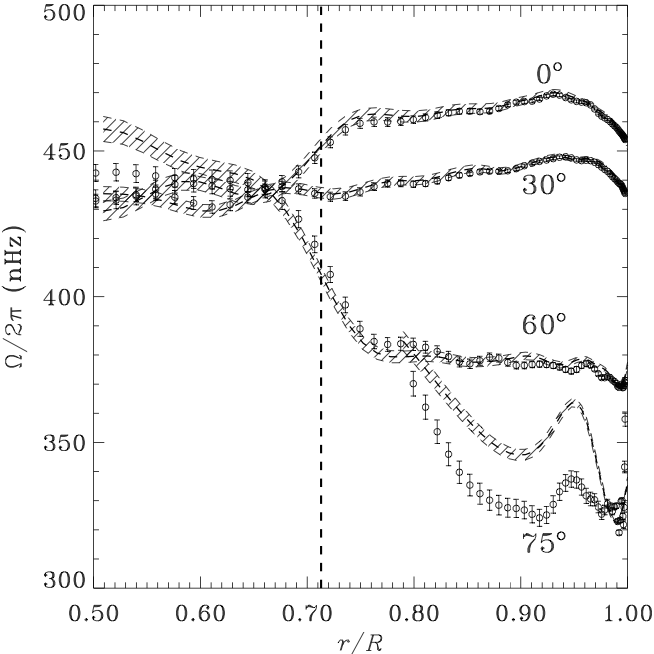
\includegraphics[keepaspectratio,width=0.45\textwidth]{invertedrotation}
\caption{Inversione della velocit\'a di rotazione a diverse latitudini. La linea verticale tratteggiata indica la base della zona convettiva. Da \cite{chr02helioseismology}.}
\end{figure}

%Per inversione 2D, cio\'e che considera la dipendenza generica $\Omega(r,\theta)$, si esprimono direttamente le differenze in frequenze:
\begin{equation}
\omega_{nlm}-\omega_{nl0}=m\int_0^R\int_0^{\pi}K_{nlm}(r,\theta)\Omega(r,\theta)r\,dr\,d\theta\label{eq:invrot2D}
\end{equation}

%mentre nel caso si abbiano i coefficienti $a_{2s+1}$, scrivo la velocit\'a angolare nella forma
%\begin{equation}
%\Omega(r,\theta)=\sum_{s=0}^{s_m}\Omega_{s}(r)\psi_{2s}(\cos{\theta})\label{eq:angularv15}
%\end{equation}
%dove $\psi_{2s}$ sono polinomi opportuni.

%Esiste una funzione opportuna $K_{nls}^{s}(r)$ tale che
%\begin{equation}
%2\pi a_{2j+1}(n,l)=\int_0^R\int_0^{\pi}K_{nls}^{s}(r)\Omega_s(r)\,dr
%\end{equation}
%e quindi \'e possibile determinare $\Omega_s(r)$.
\end{frame}

\section{Vincoli al modello solare dalle osservazioni sismologiche.} %%chapter: vincoli al modello solare: HCSM.

\begin{frame}{Inversione profilo velocit\'a del suono}

%La figura \ref{fig:deltacwu} mostra che un modello solare con composizione GS98, meno accurata di AGSS09, riproduce il profilo di $c_s$ in maniera pi\'u accurata: ci\'o pu\'o indicare un'opacit\'a da incrementare nel modello. Analogamente la diminuzione dell'opacit\'a diminuisce il gradiente termico nella regione radiativa quindi a pari luminosit\'a si ha un contenuto di idrogeno maggiore.

\begin{figure}[!ht]%{r}{0.5\textwidth}
        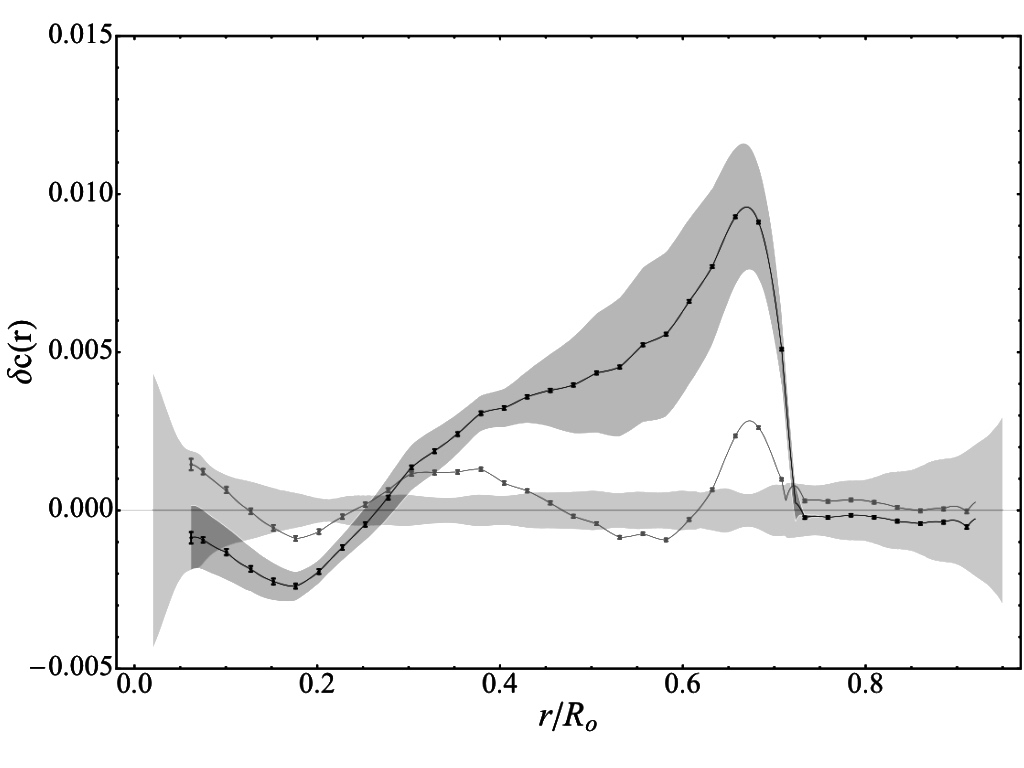
\includegraphics[width=0.9\textwidth,keepaspectratio]{deltacwu}
        \caption{%Differenza relativa nel profilo di $c_s$ risultanei dall'inversione delle differenze in frequenza tra Sole e modello: la linea chiara si riferisce alle frequenze di un modello con composzione GS98, la linea scura a composizione AGSS09. La banda chiara mostra l'errore inerente l'inversione eliosismologica, la banda scura l'incertezza a $1\sigma$ sul profilo di $c_s$ predetto dal modello. 
Da \cite{villante2014chemical}.}\label{fig:deltacwu}
\end{figure}

\end{frame}

\begin{frame}{Inversione caratteristiche zona convettiva}

%L'inversione di $c_s$ o $\rho$ mostra se un modello solare riproduce accuratamente la posizione della base della zona convettiva in quanto nella zona convettiva si ha gradiente adiabtico maggiore del gradiente radiativo; diminuzione di opacit\'a, nel caso determinata da una minore metallicit\'a, sposta la base della zona convettiva pi\'u in alto come da tabella \ref{tab:CZZvar}.

\begin{table}[!ht]%{r}{0.7\textwidth}

\pgfplotstabletypeset[
math/.style={%
        preproc cell content/.append style={/pgfplots/table/@cell content/.add={$}{$}},
    },
every head row/.style={
 before row={\toprule
 %&\multicolumn{4}{c|}{Primordiale}
 },
 every last row/.style={after row=\bottomrule},
 after row={\midrule}
},
every last row/.style={after row=\bottomrule},
every first column/.style={column type/.add={|}{}},
every last column/.style={column type/.add={}{|}},
%columns/0/.style = {column type/.add={|}{}},
display columns/0/.style={column name={Composizione}},
display columns/1/.style={column name={$Z/X$}},
display columns/2/.style={column name={$R_{CZ}$}},
display columns/3/.style={column name={$Y_{CZ}$}},
display columns/4/.style={column name={$Y_0$}},
create on use/comp/.style={create col/set list={
inversione,GS98,AGS05,AGSS09,C+11}},
columns/comp/.style = {column type/.add={|}{}},
columns/comp/.style={string type},
columns/ZX/.style={string type},
columns/ZX/.append style={math},
columns/RCZ/.style={string type},
columns/RCZ/.append style={math},
columns/YCZ/.style={string type},
columns/YCZ/.append style={math},
columns/Y0/.style={string type},
columns/Y0/.append style={math},
columns={comp,ZX,RCZ,YCZ,Y0},
%/pgf/number format/precision=4
     ]{CZvsZ.txt} %%%
     \caption{Caratteristiche della zona convettiva: confronto tra valore eliosismologico e valore ricavato da modello solare con diverse metallicit\'a del raggio della base della zona convettiva $R_{CZ}$, dell'abbondanza di elio superficiale $Y_{CZ}$ e dell'abbondanza di elio primordiale. Da \cite{basu2016global}.}
\label{tab:CZZvar}
\end{table}

\end{frame}
